\subsubsection{Giới thiệu}
Mạng thần kinh tích chập được phát triển dựa trên thí nghiệm của Hubel và Wiesel về vỏ não thị giác của mèo. Thí nghiệm này đã chỉ ra trong vỏ não thị giác của mèo có các vùng tế bào tương ứng với các vùng nhìn thấy của mắt, nghĩa là các vùng nhìn thấy khác nhau sẽ kích hoạt các vùng tế bào tương ứng của chúng. Ngoài ra thí nghiệm cũng cho thấy có một vài tế bào thì nhạy cảm hơn với các cạnh thẳng, trong khi các tế bào khác thì không. Các tế bào thần kinh này nối với nhau thành một hệ thống thần kinh sinh học hoàn chỉnh. Chính điều này đã khiến các nhà khoa học thiết kế ra mạng thần kinh tích chập với những đặc điểm giống hệ thần kinh thị giác, với hình ảnh thực được mắt nhìn thấy được thay bằng dữ liệu đầu vào có cấu trúc lưới (\textit{grid-structured}), nghĩa là dữ liệu mà vị trí tương đối của nó so với các dữ liệu khác trong không gian là quan trọng. Ví dụ dễ thấy về dữ liệu có cấu trúc lưới là hình ảnh hai chiều, vì các pixel kề nhau thường mang màu sắc gần giống nhau, và thường nó biểu thị cho một vật thể nào đó. Bởi vì đặc trưng xử lý dữ liệu có cấu trúc lưới, do đó các dạng dữ liệu tuần tự như văn bản, chuỗi thời gian, \dots cũng có thể được xử lý bằng mạng thần kinh tích chập.\cite{Aggarwal2023-zk}

Một đặc điểm quan trọng định nghĩa mạng tích chập là phép tích chập (\textit{convolution operation}), được biểu thị dưới dạng các lớp tích chập (\textit{convolution layer}) trong mạng thần kinh. Phép tích chập là một phép nhân ma trận giữa một ma trận trọng số vuông có cấu trúc lưới, với một phần nhỏ đầu vào có cấu trúc lưới được lấy từ các phần khác nhau trong đầu vào hoàn chỉnh. Do đó, các mạng tích chập được định nghĩa là mạng thần kinh nhân tạo có sử dụng ít nhất một lớp tích chập.

Mạng tích chập hoạt động khá giống với một mạng thần kinh cơ bản. Khác biệt ở chỗ kết nối giữa các lớp trong mạng này được thiết kế để bảo toàn vị trí tương đối của dữ liệu (tính không gian của dữ liệu). Các kết nối giữa các lớp này thường không phải loại kết nối đầy đủ (\textit{fully connected}) mà là kết nối thưa (\textit{sparsely connected}). Trong mạng tích chập có ba loại lớp thường thấy: lớp tích chập (\textit{convolution layer}), lớp gộp (\textit{pooling layer}) và lớp ReLU (\textit{ReLU layer}). Lớp ReLU hoạt động như một lớp ẩn trong mạng thần kinh truyền thống.

\subsubsection{Kiến trúc cơ bản}
Trong mạng tích chập, trạng thái của các lớp được sắp xếp dựa trên cấu trúc lưới trong không gian. Vị trí dữ liệu trong cấu trúc lưới này là quan trọng, vì một nhóm cục bộ các điểm dữ liệu gần nhau trong không gian, sẽ được ánh xạ qua phép tích chập hay phép biến đổi (\textit{transformation}) để thành dữ liệu mới. Đối với mạng thần kinh nhân tạo, giá trị của mỗi lớp ẩn $\mathbf h$ là một vector hay một tensor $1$ chiều (vector), thì giá trị của mỗi lớp trong mạng tích chập là một tensor $3$ chiều, bao gồm chiều rộng (\textit{width}), chiều cao (\textit{height}) và chiều sâu (\textit{depth}). Với chiều rộng và chiều cao thường được xem là toạ độ trong cấu trúc lưới (toạ độ trong không gian), còn chiều sâu thể hiện cho một thuộc tính khác độc lập với không gian. Ví dụ một tấm hình $32\times 32$ được lưu với bảng màu RGB, thì biểu diễn của nó trong mạng tích chập là một tensor $3$ chiều $32\times 32\times 3$, với mỗi lớp $32\times 32$ là một tensor $2$ chiều tượng trưng cho ma trận vị trí, còn chiều thứ $3$ biểu diễn một kênh màu căn bản (\textit{color channel}) trong RGB. Ở đây ta ký hiệu trạng thái $\mathbf h_p$ của lớp $p$ sẽ có chiều là $L_p\times B_p\times d_p$, với $L$ là chiều dài (\textit{lenght}), $B$ là chiều rộng (\textit{breath}), $d$ là độ sâu (\textit{depth}). Với mỗi lớp tương ứng với $d=1\dots n$ ta gọi nó là bản đồ đặc trưng (\textit{feature maps}).

Đối với mạng thần kinh truyền thống hay mạng hồi quy, các tham số cạnh được biểu diễn dưới dạng ma trận, thì trong mạng tích chập các tham số này được biểu diễn dưới dạng tensor $3$ chiều, và gọi là bộ lọc (\textit{filters}). Một bộ lọc thường có chiều dài bằng chiều rộng, và ta ký hiệu là $F_q\times F_q\times d_q$. Với chiều $F_q$ có điều kiện $F_q<L_q,F_q<B_q$, $F_q$ thường là một số lẻ nhỏ, ví dụ như $3$ và $5$. Chiều sâu $d_q$ phải bằng chiều sâu của đầu vào (hay bằng chiều sâu của lớp mà bộ lọc áp dụng). Bộ lọc sẽ trượt (\textit{slide}) trên tất cả các vị trí khả dĩ của đầu vào để tạo đầu ra. Kết quả đầu ra được tính bằng cách làm phẳng (\textit{flatten}) tensor $3$ chiều $F_p\times F_p\times d_p$ của đầu vào và bộ lọc thành $2$ vector có độ lớn là $F_p\cdot F_p\cdot d_p$, rồi tính tích chấm của hai vector này, nên kết quả đầu ra sẽ là một con số (hình \ref{figure:convolution-layer}).
\begin{figure}[htb]
    \centering
    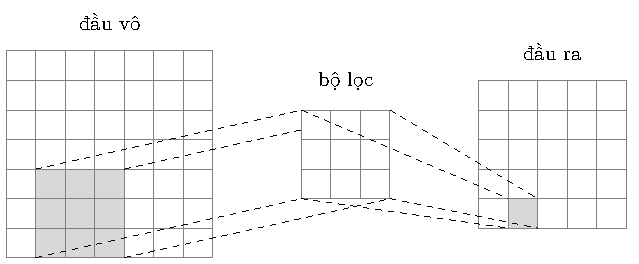
\includegraphics[width=0.7\textwidth]{tikz_image/convolution_layer.pdf}
    \caption{Lớp tích chập với $d_p=1$}
    \label{figure:convolution-layer}
\end{figure}

Có thể thấy số vị trí mà bộ lọc có thể trượt trên đầu vào chính là số chiều của đầu ra. Như trong ví dụ trên ta có chiều dài và rộng của đầu vô là $L_p=B_p=7$, còn của bộ lọc là $F_p=3$, ta có thể tính được chiều dài mới sẽ là $L_{p+1}=L_p-F_p+1=5$ và chiều rộng mới sẽ là $B_{p+1}=B_p-F_p+1=5$. Cần lưu ý vì mỗi bộ lọc sẽ làm phẳng tensor 3 chiều và tính tích chấm, nên kết quả khi bộ lọc trượt trên toàn bộ dữ liệu đầu vào sẽ là một ma trận. Trong nhiều trường hợp chúng ta muốn tạo ra nhiều bản đồ đặc trưng hơn, ta phải áp dụng nhiều bộ lọc hơn cho dữ liệu đó (hình \ref{figure:convolution-layer-multi-filters}). Độ sâu ở lớp $p+1$ sẽ là số lượng bộ lọc chúng ta áp dụng lên lớp $p$, nên tổng tham số của bộ lọc tác động lên lớp $p$ sẽ là $F_q^2\cdot d_q\cdot d_{q+1}$.
\begin{figure}[htb]
    \centering
    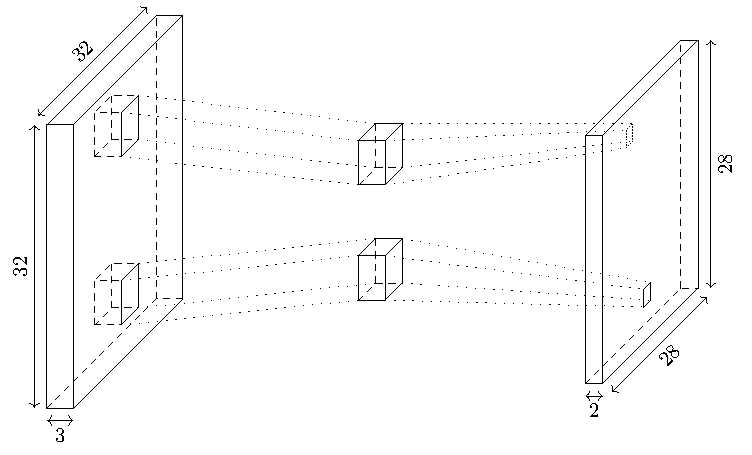
\includegraphics[width=0.7\textwidth]{tikz_image/convolution_layer_multi_filters.pdf}
    \caption{Lớp tích chập sử dụng nhiều bộ lọc}
    \label{figure:convolution-layer-multi-filters}
\end{figure}

Trong thực tế số lượng bản đồ đặc trưng trong một lớp có thể rất lớn. Lý do là vì người ta muốn áp dụng nhiều bộ lọc khác nhau để có thể xác định các mẫu không gian thuộc về một phần nhỏ của dữ liệu. Một vài bộ lọc thường dùng trong bảng \ref{table:cnn-filters}.
\begin{table}[htb!]
    \centering
    \caption{Một số bộ lọc thường dùng \cite{webpage11}}
    \label{table:cnn-filters}
    \begin{tabular}{ c c c }
        \toprule
        \textbf{Bộ lọc}              & \textbf{Giá trị}                                              & \textbf{Kết quả}                                                     \\\midrule
        Xác định (\textit{identity}) & $\begin{bmatrix}0&0&0\\0&1&0\\0&0&0\end{bmatrix}$             & 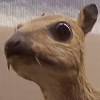
\includegraphics[width=0.2\textwidth, valign=c]{image/cnn-id.png}    \\\midrule
        Cạnh (\textit{ridge})        & $\begin{bmatrix}0&-1&0\\-1&4&-1\\0&-1&0\end{bmatrix}$         & 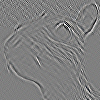
\includegraphics[width=0.2\textwidth, valign=c]{image/cnn-ed-1.png}  \\\midrule
        Cạnh (\textit{ridge})        & $\begin{bmatrix}-1&-1&-1\\-1&8&-1\\-1&-1&-1\end{bmatrix}$     & 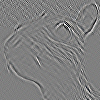
\includegraphics[width=0.2\textwidth, valign=c]{image/cnn-ed-2.png}  \\\midrule
        Sắc nét (\textit{sharpen})   & $\begin{bmatrix}0&-1&0\\-1&5&-1\\0&-1&0\end{bmatrix}$         & 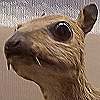
\includegraphics[width=0.2\textwidth, valign=c]{image/cnn-sharp.png} \\\midrule
        Mờ (\textit{box blur})       & $\dfrac{1}{9}\begin{bmatrix}1&1&1\\1&1&1\\1&1&1\end{bmatrix}$ & 
\includegraphics[width=0.2\textwidth, valign=c]{image/cnn-blur.png}  \\
        \bottomrule
    \end{tabular}
\end{table}

Gọi $W^{(p,q)}=[w_{ijk}^{(p,q)}]$ là bộ lọc thứ $p$ của lớp $q$, với $i,j,k$ lần lượt tương ứng với chiều dài, rộng và sâu. Gọi $H^{(q)}$ là các bản đồ đặc trưng (hay trạng thái ẩn). Phép tích chập biến đổi các bản đồ đặc trưng từ lớp $q$ đến lớp $q+1$ được định nghĩa như sau: \cite{Aggarwal2023-zk}
\begin{align}
    h_{ijp}^{(q+1)}=\sum_{r=1}^{F_q}\sum_{s=1}^{F_q}\sum_{k=1}^{d_q} w_{rsk}^{(p,q)}\cdot h_{i+r-1,j+s-1,k}^{(q)} & \quad\forall i\in\{1,\dots,L_q-F_q+1\}           \\
                                                                                                                  & \quad\forall i\in\{1,\dots,B_q-F_q+1\} \nonumber \\
                                                                                                                  & \quad\forall i\in\{1,\dots,d_{q+1}\}   \nonumber
\end{align}

Một tính chất của phép tích chập là khi ta dịch chuyển (\textit{shift}) các điểm theo một hướng nào đó $1$ đơn vị, rồi áp dụng phép tích chập, thì kết quả của phép tích chập cũng bị dịch chuyển. Nghĩa là vị trí tương đối của dữ liệu đối với nhau là không thay đổi.

Nếu ta chỉ dùng các bộ lọc $3\times 3$, thì số điểm dữ liệu đầu vào qua lớp tích chập đầu tiên là $3\times 3$, qua lớp tích chập thứ hai là $5\times 5$, qua lớp tích chập thứ ba là $7\times 7$, \dots Qua càng nhiều lớp tích chập thì độ lớn từng chiều của dữ liệu ngày càng nhỏ lại. Các lớp phía sau tuy sẽ mất dần dữ liệu nhưng những dữ liệu còn lại là sự tổ hợp của các hình mẫu đơn giản và quan trọng được trích xuất ở các lớp phía trước, quá trình này gọi là trích xuất thuộc tính phân cấp (\textit{hierarchical feature engineering}).

\subsubsection{Đệm - \textit{(Padding)}}
Xét một điểm có toạ độ không gian ở giữa dữ liệu $(L_q/2,B_q/2)$, một bộ lọc sẽ đi qua điểm này $F_q\times F_q$ lần. Nhưng đối với các điểm ở cạnh hay gần cạnh của dữ liệu, bộ lọc sẽ đi qua với số lần ít hơn, như đối với các điểm góc thì bộ lọc chỉ đi qua duy nhất $1$ lần. Điều này nói lên rằng phép tích chập truyền thống sẽ xem nhẹ các điểm ở gần các cạnh so với các điểm ở trung tâm. Vấn đề này được giải quyết bằng cách thêm các điểm dữ liệu rỗng bao quanh bên ngoài bộ dữ liệu cũ, và gọi các điểm dữ liệu mới này là phần đệm (\textit{padding}). Phần đệm được đánh số là $0$ nên nó không tham gia vào biến đổi dữ liệu. Có ba loại đệm thường thấy là
\begin{enumerate}
    \item Đệm hợp lệ (\textit{valid padding}): không thêm phần đệm, giống như cách xử lý ở phần trước. Kết quả của phép tích chập sẽ giảm số chiều còn $(L_q-F_q+1,B_q-F_q+1)$.
    \item Đệm nửa (\textit{half-padding}): phần đệm có kích thước ở mỗi cạnh là $(F_q-1)/2$ (vì $F_q$ thường là lẻ). Khi một bộ lọc đi đến viền cạnh thì gần một nửa bộ lọc sẽ đi ra ngoài phần đệm nên gọi là đệm nửa. Kết quả của phép tích chập sẽ giữ nguyên số chiều là $(L_q,B_q)$.
    \item Đệm đầy đủ (\textit{full-padding}): phần đệm có kích thước ở mỗi cạnh là $F_q-1$. Khi một bộ lọc đi đến viền cạnh thì gần hết bộ lọc sẽ đi ra ngoài phần đệm nên gọi là đệm đầy đủ. Kết quả của phép tích chập sẽ tăng số chiều lên $(L_q+F_q-1,B_q+F_q-1)$
\end{enumerate}

\begin{figure}[htb]
    \centering
    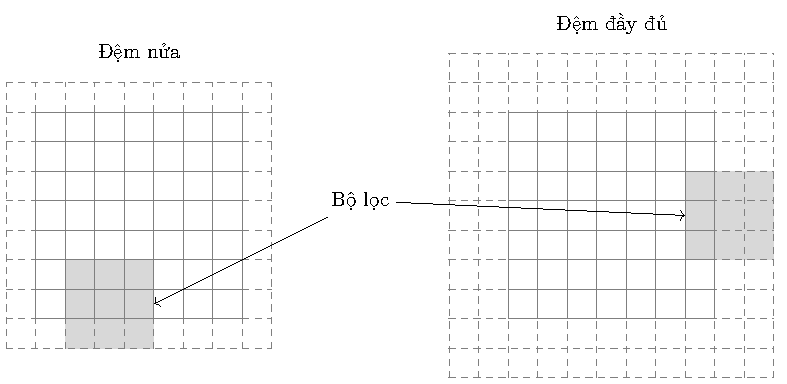
\includegraphics[width=0.7\textwidth]{tikz_image/cnn_padding.pdf}
    \caption{Đệm nửa và đệm đầy đủ}
    \label{figure:cnn-padding}
\end{figure}

\subsubsection{Bước tiến - \textit{(Strides)}}
Trong tất cả các ví dụ trên đều sử dụng bước tiến (\textit{stride}) là $1$. Trong nhiều trường hợp ta không cần phải áp dụng bộ lọc cho tất cả các điểm dữ liệu, ví dụ trong trường hợp chúng ta muốn giảm độ chi tiết của dữ liệu sau khi đi qua bộ lọc, ta có thể tinh chỉnh bước tiến lớn hơn $1$. Khi ta sử dụng bước tiến là $S_q$, bộ lọc sẽ nhận dữ liệu ở các điểm $1,S_q+1,2S_q+1,\dots$ Kích thước của đầu ra bây giờ xấp xỉ bằng $\left((L_q-F_q+1)/S_q,(B_q-F_q+1)/S_q\right)$. Ý nghĩa của điều này là đầu ra sẽ có diện tích giảm đi khoảng $S_q^2$ lần so với khi sử dụng bước tiến là $1$. Thông thường người ta chỉ sử dụng bước tiến $1$, trong một vài trường hợp đặc biệt là $2$, và rất ít khi xài bước tiến lớn hơn.

\subsubsection{Lớp ReLU}
Lớp ReLU hoạt động giống lớp kích hoạt trong mạng thần kinh truyền thống khi ta biểu diễn mạng truyền thần kinh truyền thống dưới dạng ma trận. Trong mạng truyền thống, các lớp kích hoạt và lớp tuyến tính nằm xen kẽ nhau; thì trong mạng tích chập, lớp ReLU sẽ nằm xen kẽ với các lớp tích chập và lớp gộp (\textit{pooling layer}). Việc sử dụng hàm ReLU làm hàm mặc định cho lớp này thay vì các hàm phi tuyến như sigmoid và tanh, vì hàm ReLU đã được chứng minh là tính nhanh hơn và chính xác hơn. Việc tính nhanh và chính xác hơn giúp cho việc thiết kế mạng được sâu hơn, và có thể huấn luyện mô hình trong thời gian dài.

\subsubsection{Gộp - \textit{(Pooling)}}
Phép gộp là một kỹ thuật biến một diện tích $P_q\times P_q$ ở mỗi lớp thành một số. Số chiều của kết quả sau khi gộp sẽ là $(L_q-P_q+1)\times (B_q-P_q+1)\times d_q$. Khi sử dụng bước tiến là $S_q$ với phép gộp thì số chiều sẽ khoảng $(L_q-P_q+1)/S_q\times (B_q-P_q+1)/S_q\times d_q$. Phép gộp sẽ luôn làm giảm chiều dài và rộng của dữ liệu, nhưng không bao giờ làm giảm độ sâu của nó, vì mỗi phép gộp chỉ tác động lên một lớp duy nhất một lần. Tổng quá phép gộp sẽ biến mỗi bản đồ đặc trưng cha thành bản đồ đặc trưng con nhỏ hơn mang những thuộc tính của cha.
\begin{figure}[htb]
    \centering
    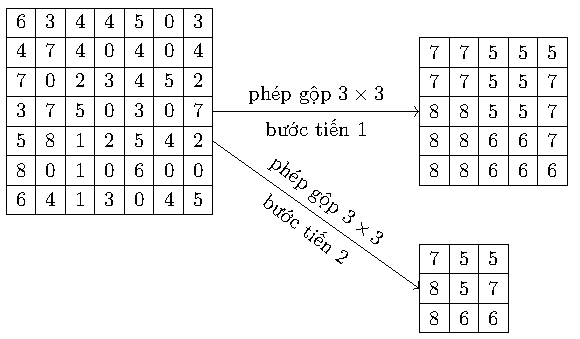
\includegraphics[width=0.5\textwidth]{tikz_image/cnn_pooling.pdf}
    \caption[Gộp tối đa]{Gộp tối đa \cite{Aggarwal2023-zk}}
    \label{figure:cnn-pooling}
\end{figure}

Thông thường trong mạng tích chập, lớp gộp sẽ nằm sau lớp tích chập và lớp ReLU. Có hai loại phép gộp thường thấy là gộp tối đa (\textit{max pooling}) và gộp trung bình (\textit{average pooling}). Mục đích của phép gộp tối đa là nó sẽ giảm chiều nhưng vẫn giữ lại các đặc điểm nổi trội (ví dụ như cách cạnh, các điểm sáng), điều này làm cho phép gộp tối đa đảm bảo được tính bất biến khi tịnh tiến (\textit{translation invariance}). Trong ví dụ nhận dạng quả chuối, dù cho quả chuối có nằm góc trên của hình hay góc dưới của hình, kết quả của phép gộp tối đa luôn giữ lại cách cạnh đặc trưng của quả chuối. Phép gộp trung bình thường ít được sử dụng hơn, và thường được sử dụng trong việc làm mượt (\textit{smooth}) đầu ra bằng cách tính trung bình của các đầu vào. \cite{Aggarwal2023-zk}

Mục đích của phép gộp khi làm giảm số chiều là để lớp đằng sau dù nhỏ hơn nhưng mang những thông tin quan trọng hơn. Phép gộp thường đi với bước tiến $>1$. Như trong hình \ref{figure:cnn-pooling}, khi sử dụng phép gộp $3\times 3$ với bước tiến $1$, kết quả đạt được là một bản đồ đặc trưng với rất nhiều các điểm dữ liệu trùng nhau, và khi dùng phép gộp $3\times 3$ với bước tiến là $2$, số điểm dữ liệu trùng nhau đã giảm đi đáng kể.

\subsubsection{Cách xắp xếp các lớp trong mạng thần kinh tích chập}
Trong mạng thần kinh tích chập thông thường bao gồm $3$ loại lớp tích chập C, lớp ReLU R và lớp gộp P xếp xen kẽ nhau; dữ liệu sau khi đi qua các lớp này sẽ làm phẳng và đưa vào mạng thần kinh truyền thống F. Lớp ReLU thường đi ngay sau lớp tích chập nên hai lớp này là CR. Sau nhiều nhóm lớp tích chập - ReLU sẽ là lớp gộp, ví dụ như CR-CR-CR-P. Ví dụ mạng AlexNet sẽ có dạng CR-P-CR-P-CR-CR-CR-P-F.

\subsubsection{Lan truyền ngược trong mạng thần kinh tích chập}
Đối với lớp ReLU ta có thể tính đạo hàm như trong mạng thần kinh truyền thống.

Đối với lớp gộp tối đa, trong trường hợp không có bất kỳ sự chồng chéo giữa các lớp gộp, nghĩa là mỗi điểm chỉ đi qua duy nhất $1$ lớp gộp, thì lan truyền ngược chỉ phụ thuộc vào vị trí của phần tử tối đa (hàm $\max$ được ghi trong bảng \ref{table:derivative-forward-backward}). Trong trường hợp có sự chồng chéo giữa các lớp gộp, gọi $P_1,\dots,P_r$ là tất cả các lớp gộp có đi qua điểm $h$ và tạo ra các giá trị $h_1,\dots,h_r$ ở lớp kế tiếp. Ta tính đạo hàm của tất cả $h_1,\dots,h_r$ tương ứng với $h$, rồi lấy tổng.

Đối với lớp tích chập, xét một điểm $c$ ở lớp $i$, điểm này sẽ đi qua nhiều bộ lọc, mỗi bộ lọc sẽ lướt qua điểm này nhiều lần và phụ thuộc vào số bước tiến. Gọi $S_c$ là tập hợp tất cả các điểm ở lớp $i+1$ được sinh ra mà có sự đóng góp của điểm $c$. Vì lan truyền xuôi từ $c$ đến $S_c$ là phép tích chấm của hai vector đơn giản, nếu điểm $r\in S_c$ thì đạo hàm $\partial r/\partial c=w_r$, với $w_r$ là trọng số trong lớp lọc kết nối giữa $c$ và $d$. Nếu gọi $\delta_c$ là đạo hàm của hàm mất mát đối với điểm $c$, dựa trên thuật toán lan truyền ngược ta có
\begin{align}
    \label{equation:cnn-backpropagation}
    \delta_c=\sum_{r\in S_c}w_r\cdot\delta_r
\end{align}

Sau khi tính đạo hàm mất mát đối với điểm, ta cần tính đạo hàm mất mát đối với trọng số $\partial L/\partial\mathbf w$ trong bộ lọc. Cần lưu ý là các điểm trong dữ liệu sẽ dùng chung một bộ lọc để tạo ra một lớp bản đồ đặc trưng mới, nên ta phải chú ý các trọng số được chia sẻ và lấy tổng chúng để được kết quả cuối cùng.

Xét một một phép tích chập với đầu vào $d_q=1$ và đầu ra $d_{q+1}=1$, với bộ lọc duy nhất $3\times 3\times 1$ như hình \ref{figure:cnn-backpropagation-filter-1}, không sử dụng đệm và bước tiến mặc định là $1$. Chọn một điểm $c$ bất kỳ trong dữ liệu đầu vào, khi bộ lọc lần đầu tiên đi qua nút $c$ thì vị trí tương ứng của nó trong bộ lọc là $i$, nghĩa là trọng số nối giữa điểm $c$ ở lớp $q$ và một điểm $r$ ở lớp $q+1$ là $w=i$, và theo như \ref{equation:cnn-backpropagation} thì đạo hàm tương ứng $\partial r/\partial c=i$. Bộ lọc này sẽ tiếp tục di chuyển và khi bộ lọc gặp điểm $c$ thì điểm này sẽ có vị trí tương ứng với bộ lọc được biểu diễn trong hình \ref{figure:cnn-backpropagation-filter-2}, và kết quả của ở lớp $q+1$ sẽ có vị trí tương ứng trong hình \ref{figure:cnn-backpropagation-filter-3}.
\begin{figure}[htb]
    \centering
    \begin{subfigure}[t]{0.3\textwidth}
        \centering
        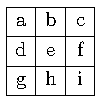
\includegraphics[width=\textwidth]{tikz_image/cnn_back_propagation_filter_1.pdf}
        \caption{Bộ lọc $3\times 3\times 1$}
        \label{figure:cnn-backpropagation-filter-1}
    \end{subfigure}\hspace{1em}
    \begin{subfigure}[t]{0.3\textwidth}
        \centering
        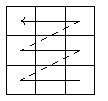
\includegraphics[width=\textwidth]{tikz_image/cnn_back_propagation_filter_2.pdf}
        \caption{Vị trí tương ứng giữa điểm $c$ và bộ lọc cùng với thứ tự xuất hiện của nó}
        \label{figure:cnn-backpropagation-filter-2}
    \end{subfigure}\hspace{1em}
    \begin{subfigure}[t]{0.3\textwidth}
        \centering
        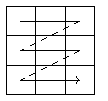
\includegraphics[width=\textwidth]{tikz_image/cnn_back_propagation_filter_3.pdf}
        \caption{Vị trí của $r$ và thứ tự xuất hiện của nó}
        \label{figure:cnn-backpropagation-filter-3}
    \end{subfigure}
    \caption{Lan truyền ngược của bộ lọc là bộ lọc}
    \label{figure:cnn-backpropagation-tensor}
\end{figure}
Nghĩa là ta có thể tạo một bộ lọc mới $3\times 3\times 1$ với các giá trị $a,b,\dots,i$ có vị trí tương ứng khi biến đổi hình \ref{figure:cnn-backpropagation-filter-2} thành hình \ref{figure:cnn-backpropagation-filter-3}. Bộ lọc này tạo thành một phép tích chập ngược từ lớp $q+1$ đến lớp $q$ và gọi là bộ lọc nghịch đảo (\textit{inverted filter}).

Xét một mạng tích chập với $d_q\neq 1$ và $d_{q+1}\neq 1$. Gọi tensor $5$ chiều $\mathcal W=[w_{ijk}^{(p,q)}]$ là bộ lọc thứ $p$ ở lớp thứ $q$, có các trọng số $w_{ijk}$ với $i\in\{1,\dots,L_q\}$, $j\in\{1,\dots,B_q\}$, $k\in\{1,\dots,d_q\}$. Gọi một tensor $5$ chiều $\mathcal U$ chứa tất cả bộ lọc nghịch đảo của $\mathcal W$ sẽ có thứ tự bộ lọc tương ứng là $k$, độ sâu của một bộ lọc tương ứng là $p$. Như trong hình \ref{figure:cnn-backpropagation-tensor} thì ta phải đảo chiều bộ lọc, nên toạ độ chiều dài và rộng tương ứng là $r=F_q-i+1$ và $s=F_q-i+1$. Mỗi phần tử trong tensor $\mathcal U$ sẽ có giá trị \cite{Aggarwal2023-zk}
\begin{align}
    u_{rsp}^{(k,q+1)}=w_{ijk}^{(p,q)}
\end{align}
